% Add as a new Numerical Results subsection after the existing placement
% subsection. Use together with 01_estimator.tex and 02_rank_selection.tex.
\subsection{Comparison with Other Structural Processing}
\label{sec:revision-structured-comparisons}

We compare six classical estimators: EM-GS, HS-GS, unstructured Rician
gradient descent, Rician gradient descent with Hankel processing, EM-GS
with smooth singular-value filtering, and the one-dimensional linearized
least-squares objective of Xu et al.~\cite{xu2025}. All methods receive
the same exact magnitude observations. The linearized method is a
comparison estimator; it does not change how the observations are generated.
The Rician gradient method uses
\begin{equation}
\mathbf G^{(t+1)}_{\rm dc}
=\mathbf G^{(t)}-
\frac{(\mathbf M^{(t)}-\mathbf Y^{(t)})\mathbf S^H}
     {\|\mathbf S\|_2^2},
\end{equation}
where $\mathbf Y^{(t)}$ is the Rician conditional field in
Section~\ref{sec:revised-estimator}. The structured version follows this
update with the same per-user Cadzow processing as HS-GS. It is an adapted
Rician--Hankel control, rather than Xu et al.'s two-dimensional projected
gradient method.

For the smooth-filtering control, each singular value $s_i$ is replaced by
\begin{equation}
\widehat s_i=\frac{s_i^3}{s_i^2+\tau^2},
\qquad
\tau=f\sqrt{\frac{1}{q}\sum_{i=1}^{q}s_i^2},
\end{equation}
where $q=r_{\max}$ and
$f\in\{0,0.05,0.1,0.2,0.4,0.8,1.6\}$.
The scale is recomputed from the current per-user Hankel spectrum in each
of the four sweeps. A zero factor bypasses filtering. This is an empirical
smooth filter, not OptShrink or a nuclear-norm solver. Each structured
method selects its own rank or factor using the same held-out squared
magnitude residual. The selected parameter is shared across users, and
the final estimate is reinitialized and fitted using all pilots.

We use $N=32$, $K=3$, $P=30$, RSR $=12$~dB,
$L\in\{3,7,14\}$ paths per user and SNRs of 0 and 10~dB. Each of the
six settings uses 400 paired trials. The iterative methods use 100 final
updates and 25 updates per candidate, with four sweeps per structural
application. These are fixed update budgets, not convergence guarantees.
The gains below compare ratio-of-sums NMSE; intervals are pointwise 95\%
paired-bootstrap intervals from 4,000 resamples.

Fig.~\ref{fig:revision-baselines} shows that HS-GS is not the best method
in every setting. Smooth filtering improves on HS-GS by
$0.623$--$1.413$~dB in five settings, with the interval above zero in each.
The remaining case, $L=3$ and SNR $=10$~dB, gives a gain of
$0.005$~dB with interval $[-0.180,0.191]$~dB.
Rician--Hankel processing improves on HS-GS by $0.171$~dB
$[0.078,0.274]$ at $L=14$ and SNR $=0$~dB, but is worse by
$0.284$ and $0.222$~dB at SNR $=10$~dB for $L=3$ and $L=7$,
respectively. The two unstructured nonlinear methods have similar NMSE
in these tests. The linearized least-squares method is less accurate than
EM-GS at all six settings under this reference strength.

An important distinction appears at $L=14$ and SNR $=0$~dB. HS-GS has
a gain of $-0.147$~dB $[-0.251,-0.046]$ over EM-GS, while smooth
filtering has a gain of $1.266$~dB $[1.152,1.380]$. Thus, a loss for
HS-GS does not show that every use of Hankel structure is unhelpful. The
observed benefit also depends on how the structure is applied and how its
parameter is selected.

\begin{figure*}[!t]
\centering
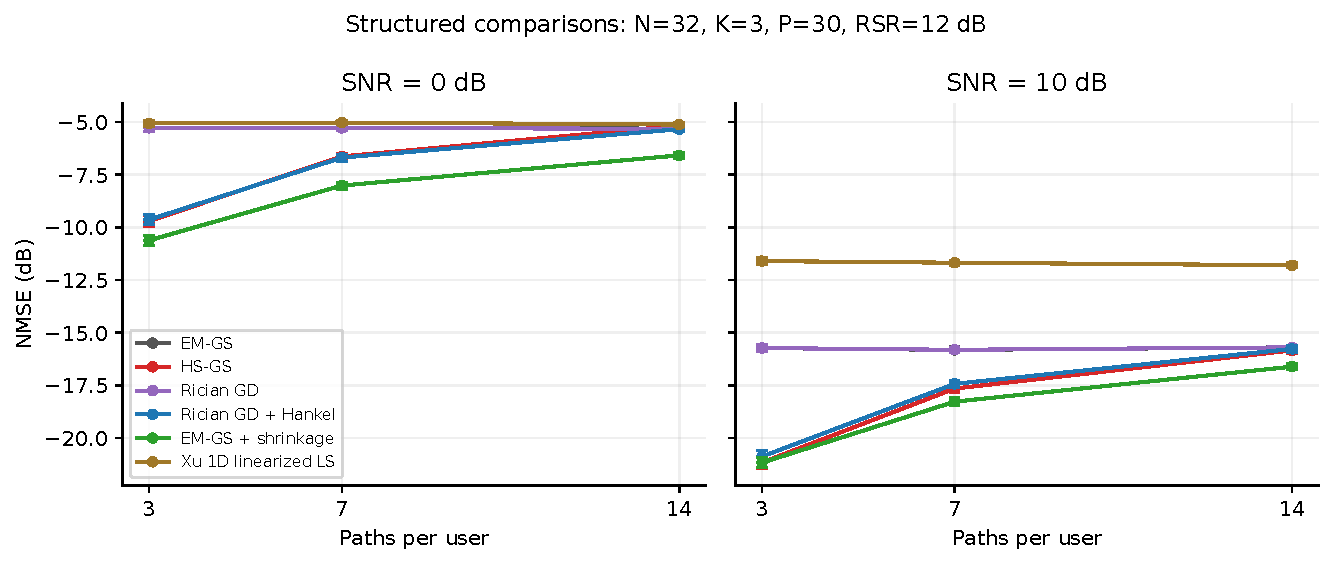
\includegraphics[width=\textwidth]{fig/revision_structured_baselines.pdf}
\caption{Six classical estimators on the same exact magnitude observations.
Each point uses 400 paired trials at $N=32$, $K=3$, $P=30$ and
RSR $=12$~dB. The two panels use SNRs of 0 and 10~dB.
Error bars are pointwise 95\% paired-bootstrap intervals.}
\label{fig:revision-baselines}
\end{figure*}
